\documentclass[../../diss.tex]{subfiles}
\begin{document}

\section{Bounded context switching for valence systems}%
\label{Section:ValenceBCS}%

In the last section, we have seen that reachability games over valence systems over graph monoids are decidable exclusively for graphs that correspond to pushdown systems.
In this section, we present a restricted version of these reachability games and conjecture that they are decidable for any underlying graph.
To justify the conjecture, we show that a similar restriction applied to the reachability problem leads to decidability in all cases.

\paragraph{Bounded context switching}

The restriction that we will consider is \emph{bounded context switching (BCS)}~\cite{QadeerR05}.
Consider a concurrent system.
A context is a part of a computation in which only one component or thread is active.
Bounding the number of context switches means that instead of each component becoming active arbitrarily often, there is a limit on how often the active component can change.
We may see a system with a BCS restriction in place as an underapproximation of the real system.
If the restricted system shows undesired behavior, \eg an error location in the source code is reachable, the same is true for the unrestricted system.
The BSC restriction is popular for two reasons.
Firstly, it has been empirically shown that bugs in concurrent systems often occur within few context switches~\cite{MusuvathiQ07,LuSSZ08}.
Secondly, the BCS restriction usually drastically improves the decidability and computational complexity of decision problems.

For example, consider multi-pushdown systems, systems that use several stacks as storage.
We may think of such a system as a concurrent system consisting of one pushdown automaton per component.
It is well known that this type of system is Turing-complete if we have at least two stacks with two stack symbols each.
Hence, reachability is undecidable~\cite{Ramalingam00}.
In a context, only a single component is active.
Hence, also just a single stack is used in a context.
Hence, the BCS restrictions limits changing the active stack.
Given a bound on the number of context switches encoded in unary, the reachability problem for the resulting model is not just decidable, but in fact $\NPTIME$-complete~\cite{QadeerR05}.

In the following, we want to define a BCS restriction for valence systems.
In the case of valence systems, there is no natural notion of thread or component.
Instead of introducing such a notion (which would then also force us to specify how the components communicate), we will base our notion of contexts exclusively on the storage.
This is inspired by the definition of BCS for multi-pushdown systems, where context switches occur when the stack that is currently used changes.

In a valence system that consists of several components, we would expect each of the components to have a storage that is independent of the part of the storage used by every other component.
Using the terminology introduced in the previous section, we would expect the storage graph to be the product of several graphs.
Each graph that is a factor of the product corresponds to the storage used by one component.

A context switch should separate parts of the computation that use independent parts of the storage.
For example, if $a \indeprel b$, then the monoid element $\inc{a}\inc{b}$ contains a context switch.
A drawback of the storage-based definition is that the notion of context switch is not invariant under the congruence $\cong$.
Hence, it is not well-defined on monoid elements, but rather on their representatives.
For example, if $a \indeprel b$, then $\inc{a}\inc{b}\dec{b}\dec{a} \cong \inc{a}\dec{a} \cong \eps$, where $\inc{a}\inc{b}\dec{b}\dec{a}$ contains two context switches, but $\inc{a}\dec{a}$ and $\eps$ contain none.
To circumvent the problems that arise from this, we redefine valence systems over graph monoids so that their configurations do not store monoid elements, but representatives.
Formally, we consider configurations from $Q \times \ops^*$ that consist of a control state and the sequence of operations that has been executed.
In a configuration $(q,m)$, we can use a transition $q \tow{m'} q'$ and move to $(q',m.m')$ if $m.m'$ represents a right-invertible monoid element.
For the reachability problem, we consider the unique initial configuration $(q_\init,\eps)$.
Solving the reachability problem is checking whether a configuration $(q_\final,m)$ with $m \cong \eps$ is reachable.
For a given finite syntactic representation of a valence system, this version of the reachability problem is equivalent to our definition from \cref{Valence:Systems}.
We have just changed the representation of the (potentially infinite) transition system arising from the finite syntax.

We come back to the definition of context switching.
For our earlier example, it seems reasonable to define a context switch to occur between two operations $\incdec{a}\incdec{b}$ if $a \indeprel b$.
However, it turns out that this definition is not restrictive enough regarding distinct nodes $a \neq b$ and too restrictive if $a = b$.
On the one hand, consider the case of a single node $a$ that has a self-loop, $a \indeprel a$.
Using operations for $a$ successively would introduce one context switch per operation and heavily limit the usability of this part of the storage.
Luckily, our definition of a context switch can avoid being so restrictive.
On the other hand, consider the graph with three nodes $a,b,c$ such that $a \indeprel b$ is the only edge.
In the sequence $\inc{a}\inc{c}\inc{b}$, no two adjacent operations are associated to nodes that are independent.
However, the sequence contains $\inc{a}$ and $\inc{b}$ and uses independent parts of the storage.
For the theory that we will develop in the rest of this section to work, we will need to see $\inc{a}\inc{c}$, $\inc{b}$ as a context switch.

The above discussion entails the following formal definition.

\begin{definition}
    A set $V' \subseteq V$ of nodes of the graph $(V,I)$ is \emph{dependent} if for any $o_1, o_2 \in V'$ with $o_1 \neq o_2$, $o_1 \notindeprel o_2$ holds.
    A set of operations is dependent if the underlying set of nodes is.
    A sequence $m \in \ops^*$ is dependent if the set of operations used in that sequence is.

    The \emph{first context} of a sequence $m \in \ops^*$ is its maximal dependent prefix.
    The decomposition into contexts is obtained inductively:
    A dependent sequence is a single context, a non-dependent sequences decomposes into its first context and the decomposition of the remaining suffix.
    The \emph{number of context switches} of a sequence is the number of \nb{contexts minus one}.
\end{definition}

\begin{figure}[t]
    \centering%
    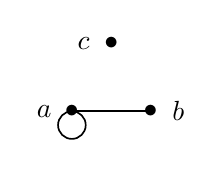
\begin{tikzpicture}[->,>=latex,node distance=1em,semithick]

\node (a) at (0,0) {$\bullet$};
\node (b) at (1,0) {$\bullet$};
\node (c) at (60:1) {$\bullet$};

\node at (0.5,-0.4) {};

\node [left of=a] {$a$};
\node [right of=b] {$b$};
\node [left of=c] {$c$};

\path [draw,-]
    (a.center) -- (b.center)
;

\draw (a.center) ++(-90:0.5em) circle (0.5em);

\end{tikzpicture}
%
    \caption{A graph for which we consider the BCS restriction.}%
    \label{Figure:ValenceBCSExampleGraph}%
\end{figure}

We demonstrate the definition on an example.
Consider a graph with the nodes $\set{a, b, c}$ and the edges $a \indeprel a$ and $a \indeprel b$.
It is depicted in \cref{Figure:ValenceBCSExampleGraph}.
Note that this graph cannot be seen as the product of several non-empty graphs.
% Nevertheless, our definition of \emph{contexts} should introduce a meaningful restriction.
Consider the sequence of operations $m = \inc{a}\inc{a}\dec{a}\inc{c}\inc{b}\dec{b}\dec{c}\inc{b}\dec{a}\dec{b}$ and note that $m \cong \eps$.
The sequence~$m$ has three context switches and consists of four contexts.
Its maximal dependent prefix is $\inc{a}\inc{a}\dec{a}\inc{c}$.
The next operation $\dec{b}$ starts a new context because $a \indeprel b$ are two distinct nodes connected by an edge.
The remaining contexts are $\inc{b}\dec{b}\dec{c}\inc{b}$, $\dec{a}$, and $\dec{b}$.

For more examples, let us consider the graphs from \cref{Figure:ValenceSystemExamples} \resp \cref{Example:ValenceSystemExamples}.
Graphs that represent pushdown systems do not contain edges, so every computation consists of a single context.
Reachability and reachability under BCS coincide.
For graphs that represent multi-pushdown systems like the graph $C_4$, our definition of BCS coincides with the well-known definition of BCS from the literature: A context is an infix of the computation in which just one stack is active.
For graphs representing VASS or integer VASS, switching the context means using a different counter.

\paragraph{Reachability under bounded context switching}

With the notion of context switches at hand, we can formally define the BCS restriction for the reachability problem.

\begin{problem}
    \problemtitle{Valence reachability under bounded context switching}
    \probleminput{Valence system $(\graphmonoid,Q, \delta, \qinit, \qfinal)$ over graph $G$,%
    \newline%
    bound $k \in \N$ encoded in unary.}
    \problemquestion{Is there a computation $(\qinit,\eps) \to^* (\qfinal,m)$%
    \newline%
    such that $m \cong \eps$ and $m$ has at most $k$ context switches?}%
\end{problem}

We will discuss this problem in detail later.
For now, we want to focus on an extended version: valence reachability games under the BCS restriction.

\paragraph{Reachability games under bounded context switching}

We can combine the definition of valence reachability games and valence reachability under BCS into a single definition of valence reachability games under bounded context switching.
Assume we are given a game valence system over a graph monoid and a bound $k \in \N$ on the number of context switches.
The goal of the existential player is, starting from $(\qinit,\eps)$ to reach $(\qfinal,m)$ where $m \cong \eps$ represents the empty storage and has at most $k$ context switches.
Here, we use the modified semantics from earlier in which we do not just keep track of monoid elements, but instead track the sequence of operations.

When formally defining valence reachability games under BCS, we have a choice to make.
Both players can influence the number of context switches in a play of the game.
In one variant, we give the obligation of ensuring that the bound on the number of context switches is not exceeded to the existential player.
She will lose all plays that contain too many context switches.
If a play already contains the maximum number of allowed context switches, the universal player can enforce her win by choosing another context switch.
The second option is to block all transitions that introduce more than the allowed number of context switches, no matter which player is active.
The first option has the advantage that a winning strategy for the existential player in the restricted game is also a winning strategy in the game without the BCS restriction.
This is because the BCS restriction only limits the moves of the existential player, while the universal player can still react using all moves in the unrestricted game.

In the following, we will consider the second variant.
We claim that it is powerful enough to simulate the first variant.
To this end, we modify the underlying valence system so that it keeps track of the number of context switches that have already occurred and the set of dependent nodes that have been used in the current context.
The latter is needed to identify the next context switch.
For the simulation, we simply replace every transition that would introduce the $\nth{(k+1)}{st}$ context switch by an $\eps$-labeled transition that leads to a deadlock.
If in the original game, the existential player is forced to introduce a $\nth{(k+1)}{st}$ context switch or if the universal player is able to do so, the modified game will move to this deadlock state.
The final state has not been reached and the existential player loses.
Note that the game is designed so that it is impossible for a computation to have more than $k$ context switches, so applying the second restriction does not change the semantics.

We conjecture that for every graph monoid, valence reachability games over the associated graph monoid with the bounded-context-switching restriction are decidable.

\begin{conjecture}
    Reachability games on valence systems over graph monoids with BCS are decidable.
\end{conjecture}

While we have no proof for this statement, we have two reasons justifying the conjecture.
The first one is the fact that decidability has been shown in the case of games over multi-pushdown systems.
In fact, \citea{Seth09} has a shown that multi-pushdown games are decidable both with a bounded-context-switching and a bounded-phase-switching restriction.
Bounded phase switching is a weaker restriction than bounded-context switching (BCS) that allows more computations: In each phase, pushes can be executed on all stacks, but pops can only occur on a single stack.
Our definition of BCS for valence systems over graph monoids is a generalization of BCS for multi-pushdown systems.
One can hope that this also means that the decidability of reachability games generalizes from multi-pushdown games to \nb{valence games}.

Note that Seth's algorithm is rather involved.
It is a generalization of Walukiewicz's decision procedure~\cite{Walukiewicz01} for context-free games that we have discussed in \cref{Section:CFGamesRelWork}.
In fact, it can be seen as a $k$-fold application of Walukiewicz's procedure, where $k$ is the bound on the number of phases or contexts.
Hence, the procedure is $k$-fold exponential.
It has been shown that the problem of solving such games is $(k-2)\EXPTIME$-complete if $k$ is fixed~\cite{MeyerV20} and non-$\ELEMENTARY$~\cite{AtigBKS12,AtigBKS17} if $k$ is part of the input.

The second justification for our conjecture is the following result that Meyer, Zetzsche, and the author of this thesis have shown in~\cite{MeyerMZ18}.
It proves that the aforementioned non-game version of reachability in valence systems over graph monoids is always decidable if we assume a bounded number of context switches.
It even leads to an upper bound for \nb{the complexity}.

\begin{theorem}%
\label{Theorem:ValenceReachabilityBCS}%
    Valence reachability under bounded context switching is always decidable in $\NPTIME$.
\end{theorem}

The rest of this section is an outline of the proof of the above result.
We do not give the technical details, and refer the reader to the full version of the paper~\cite{MeyerMZ18a}.
Afterwards, we comment on which techniques from the proof carry over to the game setting and which do not.

\paragraph{Proof sketch for \cref{Theorem:ValenceReachabilityBCS}}

Consider a computation $(q_\init,\eps) \to^* (q_\final,m)$, where $m \in \ops^*$ consists of exactly $k$ context switches, $m = \itr{m}{1}\ldots\itr{m}{k}$.
While the number of context switches is bounded, the length of each $\itr{m}{i}$ is not.
To deal with this issue, our goal is to represent the part of the valence system that contributes to each context as a separate finite automaton.
However, this turns out to be insufficient.
There are two problems:
Firstly, a single context may contain cancellations, \ie a context may contain $\inc{a}\dec{a} \cong \eps$.
This cannot be captured by a finite automaton.
Secondly, two operations in the same context may be canceled out by operations in different contexts.
For example, we might have $m$ as above with $m \cong \eps$, where $\itr{m}{i} = \inc{a}\inc{b}$ for some $i$.
The \nb{operation $\dec{a}$} that cancels out $\inc{a}$ in $\itr{m}{i}$ may be contained in some context $j$, and the $\dec{b}$ associated to $\inc{b}$ may be contained in some other context $j'$ with $j \neq j'$.

To overcome the first problem, we restrict ourselves to irreducible contexts.
Normally, an irreducible sequence of operations is one to which we cannot apply the cancellation rule,~\RuleCancel, even after potentially applying the swapping rule,~\RuleSwap.
If we only consider contexts, the definition can be simplified.
A context contains only operations that form a dependent set and the swapping rule can never be applied to operations for distinct nodes.
Formally, a context is \emph{irreducible} if it does not contain the infix $\inc{a}.\dec{a}$ for an arbitrary symbol or $\dec{a}.\inc{a}$ for a symbol $a$ with $a \indeprel a$.

To ensure that the restriction to irreducible contexts is valid, we apply a preprocessing step.
We saturate the given valence system so that if there is a computation $(q_\init,\eps) \to^* (q_\final,m)$ with $m \cong \eps$ and at most $k$ context switches, then there is also a computation $(q_\init,\eps) \to^*(q_\final,m')$ where $m'$ additionally satisfies that its contexts are irreducible.
The saturation works by finding states $q,p,p',q'$ such that $q \tow{\inc{a}} p$, $p' \tow{\dec{a}} q'$ and there is a sequence of $\eps$-labeled transitions from $p$ to $p'$.
We then introduce a new $\eps$-labeled transition from $q$ to $q'$.
Intuitively, the new $\eps$-labeled transition allows the computation to skip the operations that would lead to a context being not irreducible.
For symbols $a$ with $a \indeprel a$, we additionally add transitions that can be used to skip a sequence of transitions of the shape $\tow{\dec{a}} \tow{\eps}^* \tow{\inc{a}}$.
This process is repeated exhaustively, until no new transitions are added.
Adding an $\eps$-transition might lead to another transition being added in the next iteration, but since we only add transitions but no control states, the process terminates after at most a quadratic number of steps.

We come back to the first problem.
The different operations in some fixed contexts might cancel out (or get canceled out by) operations in different contexts.
To this end, we consider block decompositions and block-wise reductions.
A block decomposition is decomposition of the irreducible contexts into infixes, \eg $\itr{m}{i} = \itr{m}{i,1} \ldots \itr{m}{i,k}$.
A block-wise reduction is a proof of $m \cong \eps$ that uses modified reduction rules.
The rules for cancellation and swapping, \RuleCancel~and \RuleSwap, work on individual operations in a sequence.
The block-wise reduction rules work on blocks of operations.
A block $\itr{m}{i,j}$ is canceled by $\itr{m}{s,t}$ if $\itr{m}{s,t}$ is a representative for the right inverse of $\itr{m}{i,j}$.
A block $\itr{m}{i,j}$ can be swapped with $\itr{m}{s,t}$ if for every operation $\incdec{o}$ in $\itr{m}{i,j}$ and every operation $\incdec{u}$ in $\itr{m}{s,t}$, $o \indeprel u$ holds.

Assume we are given a sequence $m$ and a decomposition into blocks.
Requiring that there is a block-wise reduction showing $m \cong \eps$ is a  property that is strictly stronger than just requiring $m \cong \eps$.
Consider $m = \inc{a}\inc{b}\dec{b}\dec{a}$ and the block decomposition $\inc{a}\inc{b}$, $\dec{b}$, $\dec{a}$.
We have $m \cong \eps$, but there is no block-wise reduction to $\eps$ since $\inc{a}\inc{b}$ is neither canceled by $\dec{b}$ nor by $\dec{a}$.
We have that if $m \cong \eps$, then $m$ admits a block-wise reduction to $\eps$ if we decompose it into blocks of length one that consists of single operations.
In this case, the block reduction rules are equal to \RuleCancel~and \RuleSwap.

The crucial result that we need for our algorithm is the following.
Consider a sequence $m$ with $m \cong \eps$ consisting of $k$ irreducible contexts.
Each of the $k$ contexts can be decomposed into at most $k$ blocks so that the resulting block decomposition of $m$ admits a block-wise reduction to~$\eps$.
To prove the result, we observe that for each pair of contexts $\itr{m}{i}$ and $\itr{m}{s}$, there is at most one infix of each block such that the two infixes cancel each other out using \RuleCancel.

This result gives us a quadratic bound on the number of blocks in a block decomposition, but it does not give us a bound on the length of each block.
To deal with the latter, we represent blocks by finite automata that generate these blocks as elements of their language.
As a consequence, we will not execute a block-wise decomposition on concrete blocks\footnote{Pun intended.}, but on automata representing such blocks.
Imitating the swapping rule is easy.
The automata use the \nb{operations $\incdec{o}$} as the letters of their alphabet.
Two automata can be swapped if for every operation $\incdec{o}$ in the alphabet of the first automaton and every operation $\incdec{u}$ in the alphabet of the second one, $o \indeprel u$ holds.

The cancellation rule is a bit more complicated.
Firstly, we note that if a block of an irreducible context $\itr{m}{i,j}$ has a right inverse, then this right inverse can be constructed in a \emph{syntactic} way, namely by reversing the order of $\itr{m}{i,j}$ and by swapping the polarity of the operations.
The latter means we replace $\inc{o}$ by $\dec{o}$ and vice versa.
Two automata cancel each other if the first one generates a word $\itr{m}{i,j}$ and the second one generates the syntactic right inverse of that word.
To check this property, we apply the syntactic inverse operations to the second automaton, \ie we reverse its order and swap the polarity of all transition labels.
Then, we check intersection emptiness.

\paragraph{The algorithm}

We have gathered all prerequisites to outline the procedure that decides valence reachability under bounded context switching in $\NPTIME$.
Assume we are given a valence system and a bound $k-1$ on the number of context switches, \ie we can assume that we have $k$ contexts.

\begin{enumerate}
    \item
        For each of the $k$ contexts, guess a dependent set of nodes.
        We will assume that each context will just use operations from that set.
        Construct for each context a version of the valence system in which the transitions whose label is $\inc{o}$ or $\dec{o}$ for a node $o$ not in the corresponding set are discarded.
    \item
        Apply saturation to these valence systems.
    \item
        For each $j = 1, \ldots, k^2-1$ (each index of a block in the decomposition), guess a control-state $q_j$ of the valence systems.
        Intuitively, the operations in the $\nth{j}$ block of the decomposition leads from control state $q_j$ to $q_{j+1}$, with $q_0 = q_\init$ and $q_{k^2} = q_\final$.
        Guess for each block $j$ a subset of the nodes of the context to which block $j$ belongs.
        Construct a version of the valence system in which the operations for other nodes are removed as in Step~1.
    \item
        For each $j = 0, \ldots, k^2-1$:
        See the valence system for the $\nth{j}$ block as a finite automaton $A_j$ with $q_j$ as the initial and $q_{j+1}$ as the final state.
    \item
        Consider the sequence of the automata $A_0, \ldots, A_{k^2-1}$ resulting from the previous step.
        Guess a block-wise reduction and verify that it reduces the sequence of automata to $\eps$.
\end{enumerate}

The first step is self-explanatory.
The second step ensures that if we can reach the final state with empty storage, then we can do so with a sequence of operations with irreducible contexts.

It might seem weird that we first guess a subset of nodes for each context, and later guess another subset for each block.
This is needed because when verifying the usage of swap rules in the block-wise decomposition, we need to make sure that for two blocks that we want to swap, all operations used in the first block commute with all operations in the second block.
Hence, we need to discard all operations that might appear in the context, but not in that specific block.

In Step~4., each automaton represents a language that contains a block $\itr{m}{i,j}$ of the block decomposition.
When guessing the decomposition, we guess in each step which kind of rule should be applied (cancel or swap), and to which two blocks $\itr{m}{i,j}$ and $\itr{m}{s,t}$ it should be applied.
We then verify that it is valid and that it indeed reduces the sequence to $\eps$.
It is not hard to see that a single step of the block-wise reduction can be guessed and verified in polynomial time.
To conclude that the whole procedure is in $\NPTIME$, note that the number of cancellation steps is exactly $\frac{k^2}{2}$, and that between two cancellation steps, the number of swapping steps is at most the number of remaining blocks squared.

This completes our proof sketch for \cref{Theorem:ValenceReachabilityBCS}.
We refer to the full version of the paper~\cite{MeyerMZ18a} for details.

In addition to the full proof, the paper~\cite{MeyerMZ18,MeyerMZ18a} also analyzes the computational complexity of solving valence reachability in more detail.
We briefly outline the results.
Recall that for a graph $G$, $\irreflexive{G}$ is a version of $G$ without any self-loops.
We have identified classes of graphs for which the problem is solvable in $\PTIME$, \ie deterministic polynomial time.
If $G$ is the graph under consideration and $\irreflexive{G}$ contains the graph $C_4$ from \cref{Figure:ValenceSystemExamplesC4} as an induced subgraph, then the problem is $\NPTIME$-complete.
Recall that $C_4$ is the graph corresponding to a multi-pushdown system with two stacks with a binary stack alphabet each.
Hence, this $\NPTIME$-completeness result corresponds to the result that reachability in multi-pushdown systems under bounded context switching is $\NPTIME$-complete.
In the case that $\irreflexive{G}$ contains the graph $P_4$ from \cref{Figure:ValenceSystemExamplesP4} as an induced subgraph, we were not able to determine the precise complexity of valence reachability under the BCS restriction.
We could neither prove that the problem is $\NPTIME$-complete, which would imply that our algorithm is optimal, nor provide a better algorithm that solves the problem in deterministic polynomial time.

Another open problem is a generalization of the aforementioned \emph{bounded phase switching} restriction to valence systems.
A phase of the computation of a multi-pushdown system is an infix of the computation in which the system pushes only onto a single stack.
However, the system can pop from all stacks.
Correspondingly, it seems sensible to define a phase of the computation of a valence system as a sequence of operations in which only the positive operations have to be dependent.
For multi-pushdown systems, reachability under bounded phase switching is $\NPTIME$-complete like reachability under BCS~\cite{TorreMP07}, and games with the bounded-phase-switching restriction can be solved in (deterministic) $k$-$\EXPTIME$ time for a fixed $k$~\cite{Seth09}.
We would expect that these results can be generalized to valence systems under a bounded-phase-switching restriction.
However, it is not clear how the above proof, in particular the saturation step and block decompositions, would generalize to bounded phase switching.
We leave this for future work.


In the time since the publication of our paper~\cite{MeyerMZ18}, \citea{ShettyKZ21} have generalized our result to reachability under \emph{scope boundedness}.
This notion was originally introduced for multi-pushdown systems by \citea{TorreNP20}.
For a fixed bound~$k$, a computation of a multi-pushdown is $k$-scope-bounded if after pushing each symbol onto some stack, there are at most $k$ contexts that use this stack until the symbol is popped again.
This restriction is a generalization of bounded context switching: A computation that contains at most $k$ contexts is necessarily $k$-scope-bounded.
In contrast to bounded context switching, a computation of a multi-pushdown can be $k$-scope-bounded while still containing infinitely many contexts.
Scope boundedness seems to be incomparable in expressive power to the aforementioned bounded-phase-switching restriction.

The first contribution of the paper~\cite{ShettyKZ21} is to generalize the notion of scope boundedness from multi-pushdown systems to arbitrary valence systems.
Then, the authors prove that reachability under scope boundedness can always be solved in $\PSPACE$ and they provide a classification result, showing $\PSPACE$-completeness in many cases.
This matches the $\PSPACE$-completeness for multi-pushdown systems~\cite{TorreNP20}.
The complexity-theoretic results show that the increased expressiveness of scope boundedness over bounded context switching comes with a penalty as the computational complexity rises from $\NPTIME$ to $\PSPACE$.
The techniques used in~\cite{ShettyKZ21} to prove the results include generalization of some of the concepts that we used in our study of bounded context switching, including block decompositions and \nb{block-wise reductions}.

\paragraph{From systems to games}

In the rest of this section, we explain the difficulties that arise when trying to lift the proof of decidability in valence systems under the BCS~restriction to games.
In the proof, we have implicitly used several times that the nondeterminism in the system is under the control of a single entity:
Our algorithm guesses the set of operations that will be used in each block, and a witness of reachability can only be found if the guesses are correct.
This means the entity controlling the nondeterminism in the system can be assumed to be the same entity that controls the nondeterminism in the algorithm for checking reachability.
Additionally, when we saturate a valence system, we insert transitions and hence introduce nondeterministic choices.
The transitions that are inserted by the saturation procedure do not hurt the correctness, since we can assume that the entity resolving the nondeterminism has perfect foresight:
When taking a transition labeled by $\inc{a}$, it already knows that it will then take a sequence of $\eps$-labeled transitions followed by a $\dec{a}$ transition, and nobody else can interfere with that plan.
Hence, it can directly take the $\eps$-labeled transition introduced by saturation that skips this part of the computation.

In a game setting, both tricks do not work anymore.
A nondeterministic algorithm cannot simply guess a set of operations for each block, and restrict a part of the game to that set of operations.
Intuitively, the nondeterminism in the algorithm corresponds to one of the players.
If the other player wants to use an operation that is not in this set, we cannot simply deny her this opportunity without affecting the semantics of the game.
Similarly, the saturation does not carry over if we consider a set of states that are not owned by a single player:
After taking an $\inc{a}$-labeled transition, the other player may become active, so it is not clear to the player who chose $\inc{a}$ whether a $\dec{a}$ transition will follow later.
Allowing the player to take a transition that was inserted by the saturation means that she could skip moves of the opponent, which affects the semantics of the game.

Walukiewicz's reduction~\cite{Walukiewicz01}, originally designed for context-free games (see~\cref{Section:CFGamesRelWork}), but also used by~\citea{Seth09} for multi-pushdown games with a BCS restriction, offers a way to resolve these issues.
For example, instead of letting the algorithm guess sets of nodes, this mechanism could be incorporated into the game using a negotiation mechanism:
% To be precise, the players negotiate the needed information during the play:
The existential player proposes a prediction, then the other player can either accept it -- which means she loses if she violates the prediction -- or she can challenge it, in which case she wins if and only if she can enforce a violation of the prediction.

Even with this technique at hand, trying to obtain a decision procedure for valence reachability games has turned out to be very involved.
Firstly, our result that bounds the length of a block decomposition requires all contexts of the computation to be irreducible.
It is not clear whether the saturation procedure can be lifted to the game setting.
If not, it might be possible to design a negotiation mechanism à la Walukiewicz to ensure irreducible contexts, but this seems to be quite intricate.

Assume we could successfully overcome these problems.
In Step~4.~of the algorithm, instead of a sequence of automata, we would now have to deal with a sequence of games.
It is not clear how a block-wise reduction could be conducted on the level of games.
We leave solving these problems for future work.

\end{document}
